\chapter{Background}

\section{Reinforcement Learning}

Reinforcement Learning (RL) is a branch of machine learning, alongside supervised learning and unsupervised learning, that defines a set of algorithms meant to learn how to act in a specific environment without the need of labelled data to learn from. 

The algorithm defines the agent that learns a given task, for example, walking, driving and playing a game, by trial and error, while interacting with an environment which can be real or simulated. Whenever the agent makes a set of good actions it receives a positive reward, which makes such actions more likely in the future. State, action and reward are the most important concepts in RL. The state represents the current situation of the environment. If the agent is a humanoid robot and the task is walking, one possible state representation is the positions of its actuated joints. The action set or space in case of continouos domain, describes what the agent can do in a particular state. In the humanoid robot example above, the action space is a n-dimensional vector where each dimension represents the torque command to each of the n joint motors. Finally the reward is a measure of how good are the actions carried out by the agent. 

\begin{wrapfigure}{r}{0.6\textwidth}
  \begin{center}
    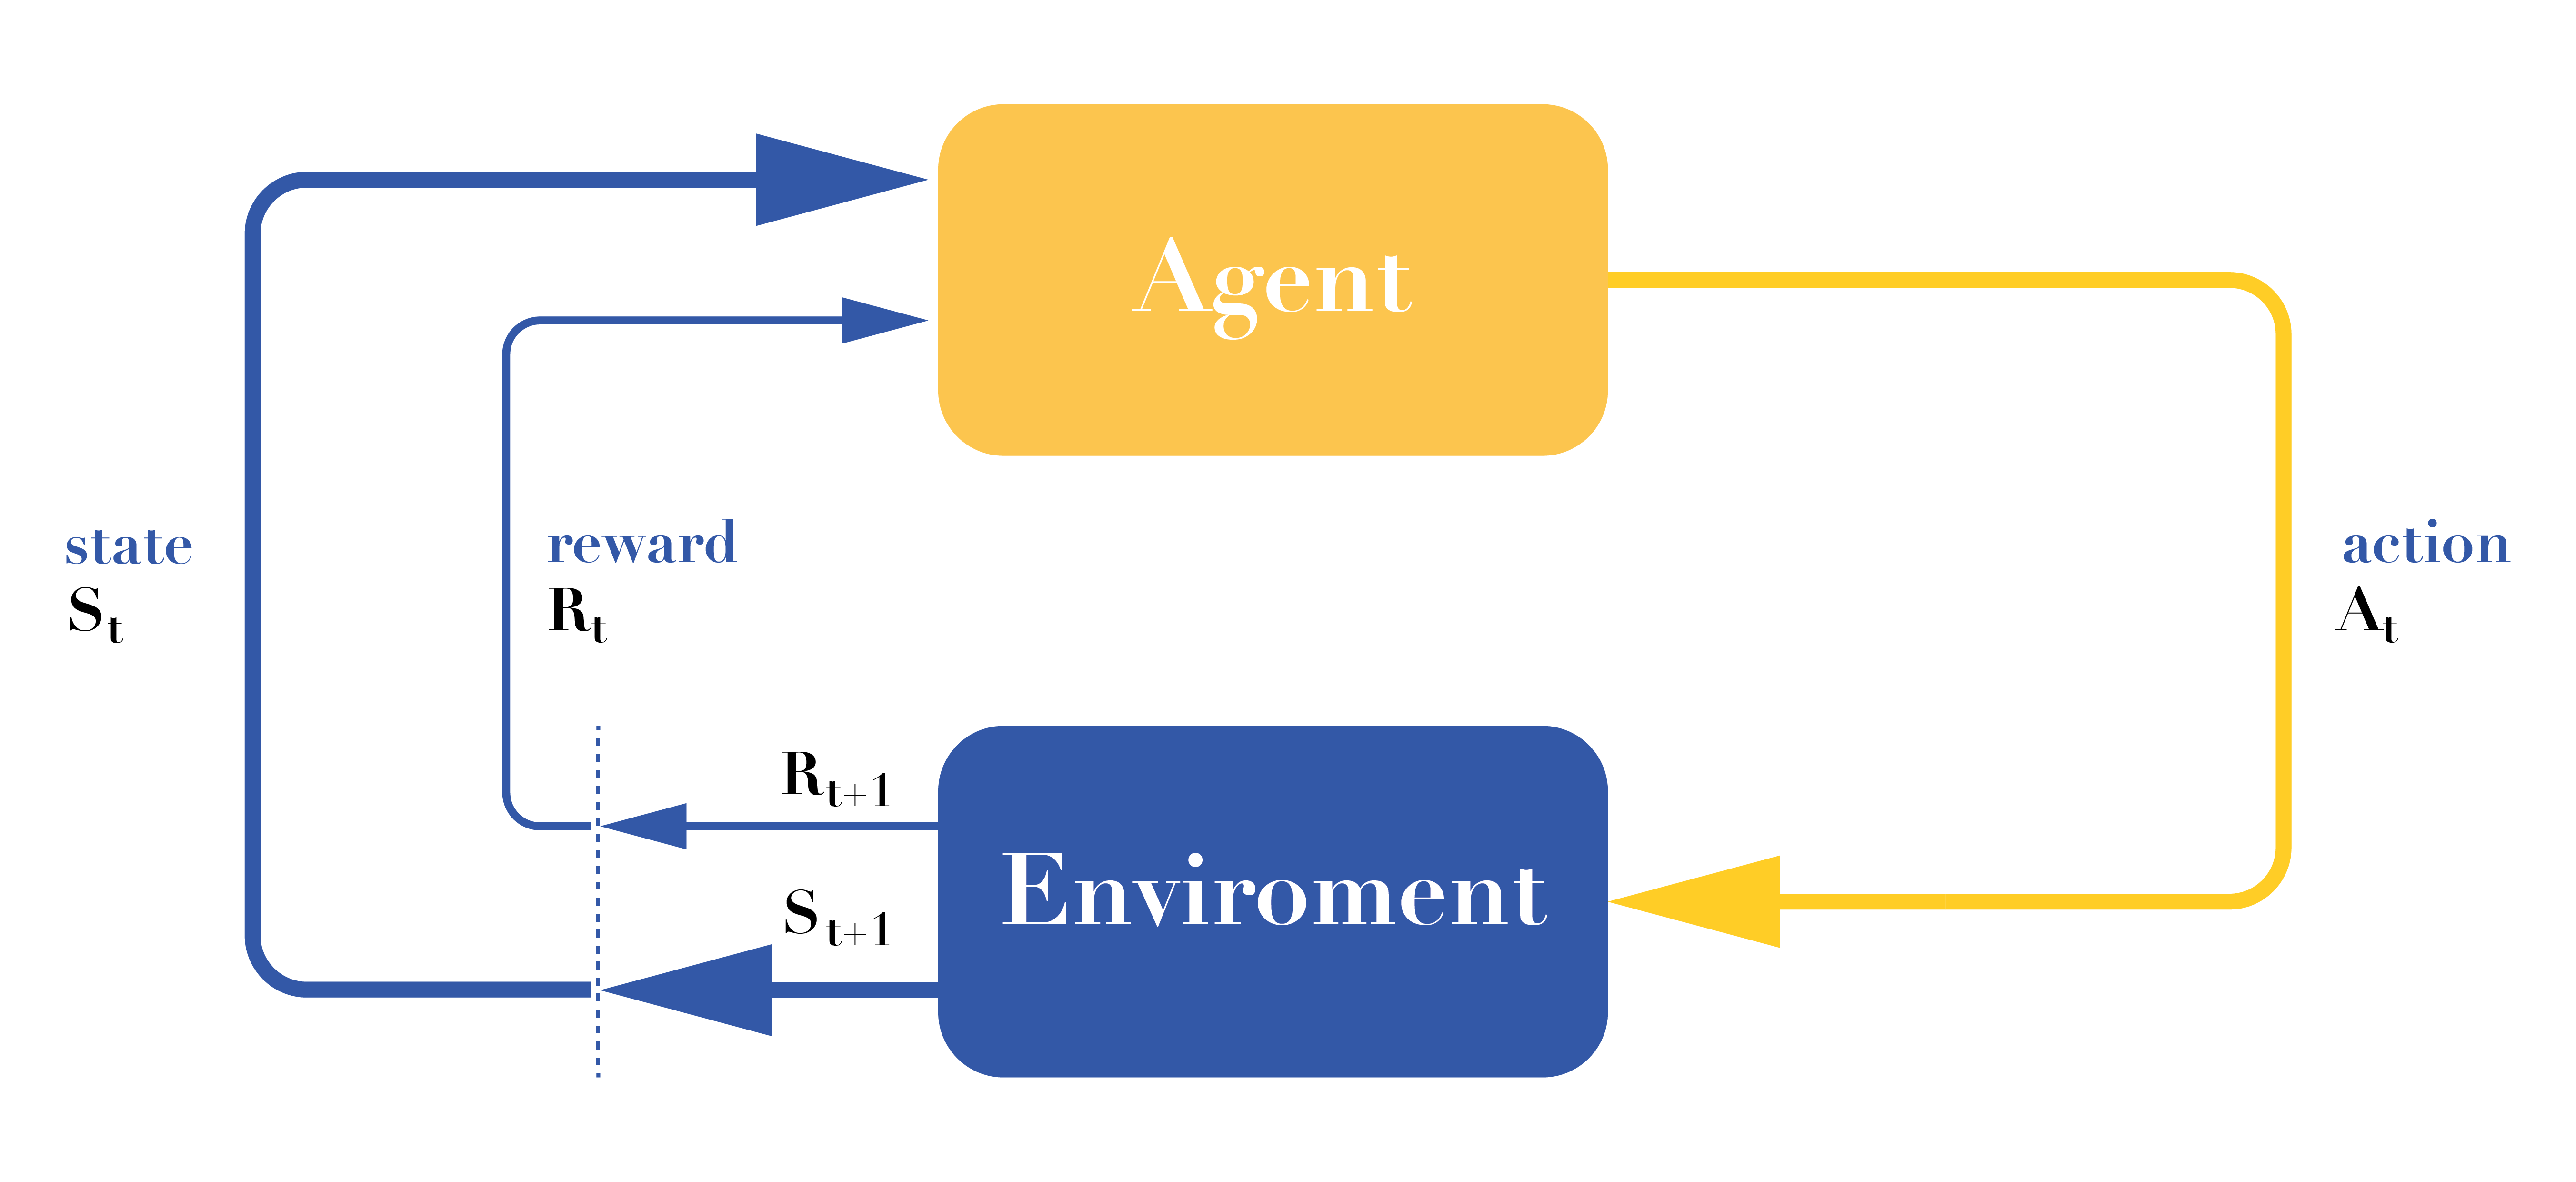
\includegraphics[width=0.6\textwidth]{background/rl.png}
  \end{center}
  \caption{Basic reinforcement learning}
  \label{fig:rl}
\end{wrapfigure}

The reward function, usually human-designed, assigns a score to the action taken by the agent. Every action that leads to a \textit{good} state increases the score and viceversa every \textit{bad} action decreases it. As described in Figure \ref{fig:rl} the agent interacts with the environment in discrete time steps. At time $t$ it gets the current state $s_{t}$ and the associated reward $r_{t}$ then the action $a_{t}$ is chosen from the set of available actions. After receiving the chosen action, the environment moves to a new state $s_{t+1}$ and the reward $r_{t+1}$ is given back to the agent. The total discounted reward to be maximized is:

\begin{equation}
  \label{eq:totalreward}
  R=\sum _{t=0}^{T}\gamma ^{t}r_{t}
\end{equation}
where $T$ is the time horizon (enventually $\infty$), $\gamma \in [0,1)$ is the discount factor which allows $R$ to be a finite value in case of $T=\infty$ and makes future rewards worth less than immediate reward. The total discounted reward function is fundamental to the agent in order to learn and optimize a policy function $\pi$:
\begin{align}
  \displaystyle \pi &:A\times S\rightarrow [0,1] &  \displaystyle \pi (a,s)&=\Pr(a_{t}=a\mid s_{t}=s) \label{eq:label1}
\end{align}
The policy is a mapping that gives the probability of taking action $a$ in state $s$. By following the policy the agent takes the action that maximizes the reward. However, the policy, especially during training, is not deterministic. This is due to one of the fundamental challenges in RL, i.e. the exploration-exploitation dilemma \citep{Sutton1998}. Indeed, the agent needs to repeat the actions it already know to be rewarding but, at the same time, it needs to explore the environment to discover actions that can lead to an even higher reward. 
The final goal of the algorithm is to learn a policy that maximizes the expected cumulative reward.
\begin{equation}
  \label{eq:rlobj}
  J(\pi)=\mathbb{E}_{\pi}[\sum _{t=0}^{T}\gamma ^{t}r(s_{t},a_{t})]
\end{equation}
There are multiple ways to learn the optimal policy $\pi^{*}(s)$. The first one is called \textit{Value iteration}, which exploits the state value function $V^{\pi}(s)$ and the action value function $Q^{\pi}(s, a)$. The state value function $V$ is the expected return starting from the state s and following the policy $\pi$:

\begin{equation}
  \label{eq:statevalue}
  V_{\pi}(s) = E_{\pi}[\sum_{t=0}^{T-1} \gamma^t r_t \mid s_t=s]
\end{equation}
while the action value function $Q$ is the expected return starting from the state s, following the policy $\pi$, taking action $a$:

\begin{equation}
  \label{eq:actionstatevalue}
  Q_{\pi}(s,a) = E_{\pi}[\sum_{t=0}^{T-1} \gamma^t r_t \mid s_t=s, a_t = a]
\end{equation}
There is an important reletionship between Equations \ref{eq:statevalue} and \ref{eq:actionstatevalue}, in fact they can be written in terms of each other:

\begin{equation}
  \label{eq:statevaluefromQ}
  V_{\pi}(s) = \sum_{a\in A} \pi(a \mid s) * Q^{\pi} (s,a)
\end{equation}

\begin{equation}
  \label{eq:actionstatevaluefromV}
  Q_{\pi}(s,a) = \sum_{s^{'}\in S} P(s^{'} \mid s,a) [r(s,a,s^{'}) + \gamma V_{\pi} (s^{'})].
\end{equation}
where P is the state transition matrix that gives the probability of reaching the next state s’ from state and $r$ is the immediate reward.

In \textit{Value Iteration}, we start from a random intialized $V$ and the algorithm, illustrasted in Listing \ref{lst:valueiteration}, repeatedly updates $Q$ and $V$ values until they converges, with the guarantee that they will converges to the optimal values.  

\begin{center}
  \begin{minipage}{0.65\linewidth}
    \lstinputlisting[escapeinside={(*}{*)}, caption=Value iteration pseudo code from \citet{Alpaydin:2014:IML:2635955}, captionpos=b, label=lst:valueiteration]{valueiteration.pseudo}
    \end{minipage}
\end{center}
Finally the policy $\pi$ can be inferred from the $Q$ function with:
\begin{equation}
  \label{eq:pifromq}
  \pi(s) = argmax_a Q(s,a)
\end{equation}
Since the agent only cares about finding the optimal policy, it could happen that the policy converges before the value function. Therefore, the so-called \textit{Policy Iteration} algorithm seeks to learn the policy directly by updating it at each step as shown in Listing \ref{lst:policyiteration}
\begin{center}
  \begin{minipage}{0.65\linewidth}
    \lstinputlisting[escapeinside={(*}{*)}, caption=Policy iteration pseudo code from \citet{Alpaydin:2014:IML:2635955}, captionpos=b, label=lst:policyiteration]{policyiteration.pseudo}
    \end{minipage}
\end{center}
Policy iteration is also guaranteed to converge to the optimal policy and it often takes less iterations to converge than the value iteration algorithm.

A major problem arises when the environment is not entirely known to the agent or is too big that is unfeasible to store all the Q and V values in a table. As well as, in the case of a continuous action space. Deep RL algorithms introduces Deep Neural Networks in order to approximate $Q$ and $V$ instead of storing them in huge tables. Function approximation allows also a better generalization of states never seen before, or with partial information, by exploiting values of similar states. 

Another important difference between RL algorithms that is worth a brief mention, is in the way the algorithm updates the policy. On-Policy methods evaluates and improve the same policy which is being used to select actions. Off-Policy methods evaluates and improve a policy that is different from the policy that is used for action selection bringing many advantages. Firstly, it allows a better exploration of new trajectories. Secondly, the agent can learn from demonstrations and finally it allows parallel learning speeding up the convergence.

\section{OpenAI Gym interface}

Gym is an open source library that defines a standard API to handle training and testing of RL agents, while providing a diverse collection of simulated environments.

\begin{wrapfigure}{r}{0.5\textwidth}
  \begin{center}
    \frame{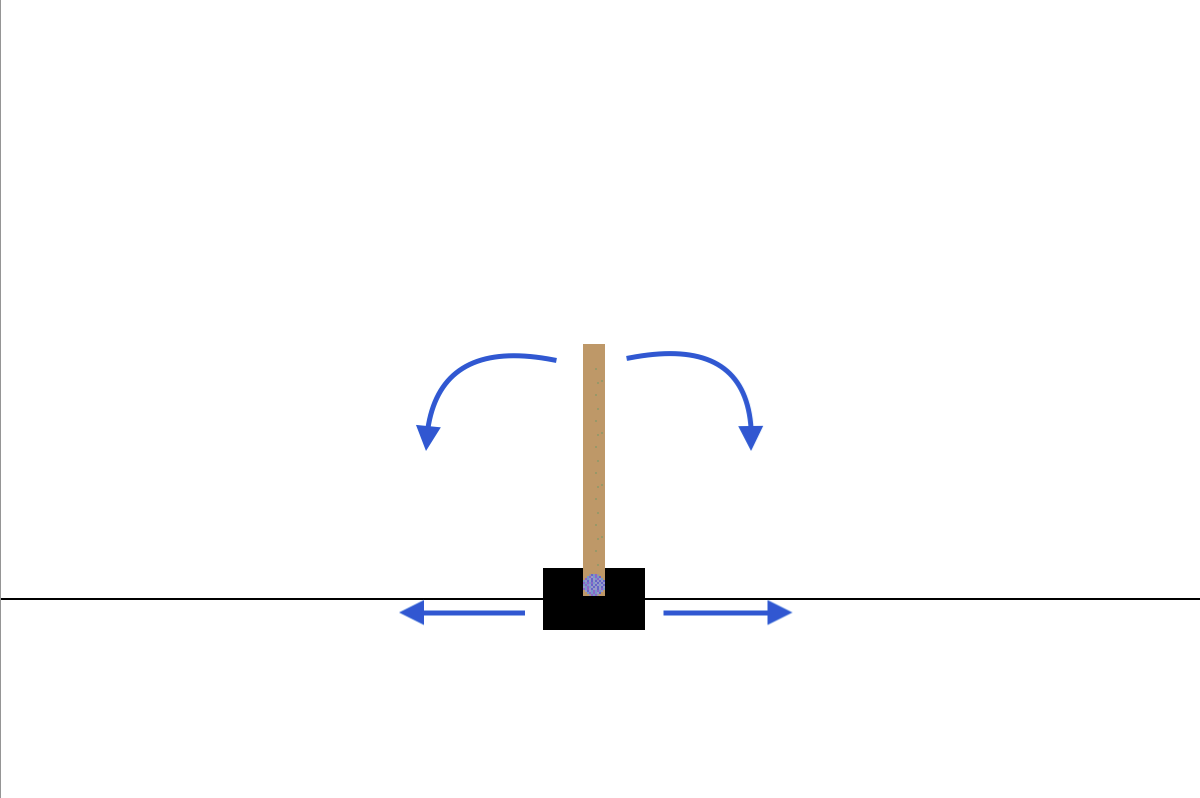
\includegraphics[width=0.5\textwidth]{background/cartpole.png}}
  \end{center}
  \caption{Cart-pole in Gym}
  \label{fig:gym}
\end{wrapfigure}
The environment is of primary importance to a RL algorithm since it defines the world of the agent in which the agent lives and operates. The standard interface designed by Gym, makes it easier to interact with environments, both made available by Gym and externally developed.
The Gym interface is simple, pythonic, and capable of representing general RL problems. Cart-pole, shown in Figure \ref{fig:gym}, is a classic example of a Gym environment. A pole is attached by an un-actuated joint to a base, which moves along a straight track. The pendulum is placed upright on the base and the goal is to balance the pole by moving the base to the left and right. The action set include two actions, move right and move left. The observation space includes the base position, the base velocity, the pole angle and the pole angular velocity.
The documentation provides a reference template shown in Listing \ref{lst:gym} that describes what are the fundamental methods a gym environment should implement to work properly.
Any exisisting environment built with Gym implements the following few methods which are enough to run any basic RL algorithm or eventually override them in case of custom environments:

\begin{center}
  \begin{minipage}{0.45\linewidth}
    \lstinputlisting[caption="Gym template", captionpos=b,  label=lst:gym]{gym.py}
    \end{minipage}
\end{center}

\begin{itemize}
  \item \textbf{init:} every environment should extend gym.Env and contain the variables\\ \textit{observation\_space} and \textit{action\_space} specifying the type of possible observations and actions using spaces.Box or spaces.Discrete.
  \item \textbf{step:} this method is the primary interface between environment and agent, it takes as input the action and return informations (observation, reward, done) about the current state.
  \item \textbf{reset:} this method resets the environment to its initial values returning the initial state of the environment.
  \item \textbf{render:} this method pops up a window rendering the environment when a parameter \textit{mode='human'} is passed.
  \item \textbf{close:} this method performs any necessary cleanup before closing the program.
\end{itemize}
Beside the environment, gym provides a set of wrappers to modify an existing environment without having to change the underlying code directily. The three main common things a wrapper wants to do are:

\begin{itemize}
  \item Transform actions before applying them to the base environment
  \item Transform observations that are returned by the base environment
  \item Transform rewards that are returned by the base environment
\end{itemize}
The given set of wrappers to reach any of the aforementioned goal includes: \textit{ActionWrapper}, \textit{ObservationWrapper}, \textit{RewardWrapper}. Alongside with more complex wrappers which che be found in the offical documentation. Furthermore, custom wrappers can be implemented by inheriting from \textit{Wrapper}.

\section{Soft Actor Critic - SAC}
The soft actor critic algorithm \citep{art:sac} illustrasted in Figure \ref{fig:sac} is a state-of-the-art RL algorithm designed to outperform prior on-policy and off-policy methods in a range of continuous control benchmark tasks. 

It aims and succeeds to reduce the sample complexity, since even relatively simple task can require millions of steps of data collection, and brittleness in convergence. A poor sample efficiency in deep RL methods may be due to on-policy learning since it requires new samples to be collected for each gradient step. In order to improve the sample efficiency, SAC draws on the maximum entropy framework. It introduces to the objective \ref{eq:rlobj} an entropy maximization term which aids stochastic policies by augmenting the objective with the expected entropy of the policy:
\begin{equation}
  J(\pi)=\mathbb{E}_{\pi}[\sum _{t=0}^{T}\gamma ^{t}r(s_{t},a_{t})+\alpha H(\pi(\cdot \mid s_{t}))]
\end{equation}
where $\alpha$ is a temperature parameter that weighs the entropy term and thus controls the policy stochasticity.


\begin{figure}[h]
  \begin{center}
    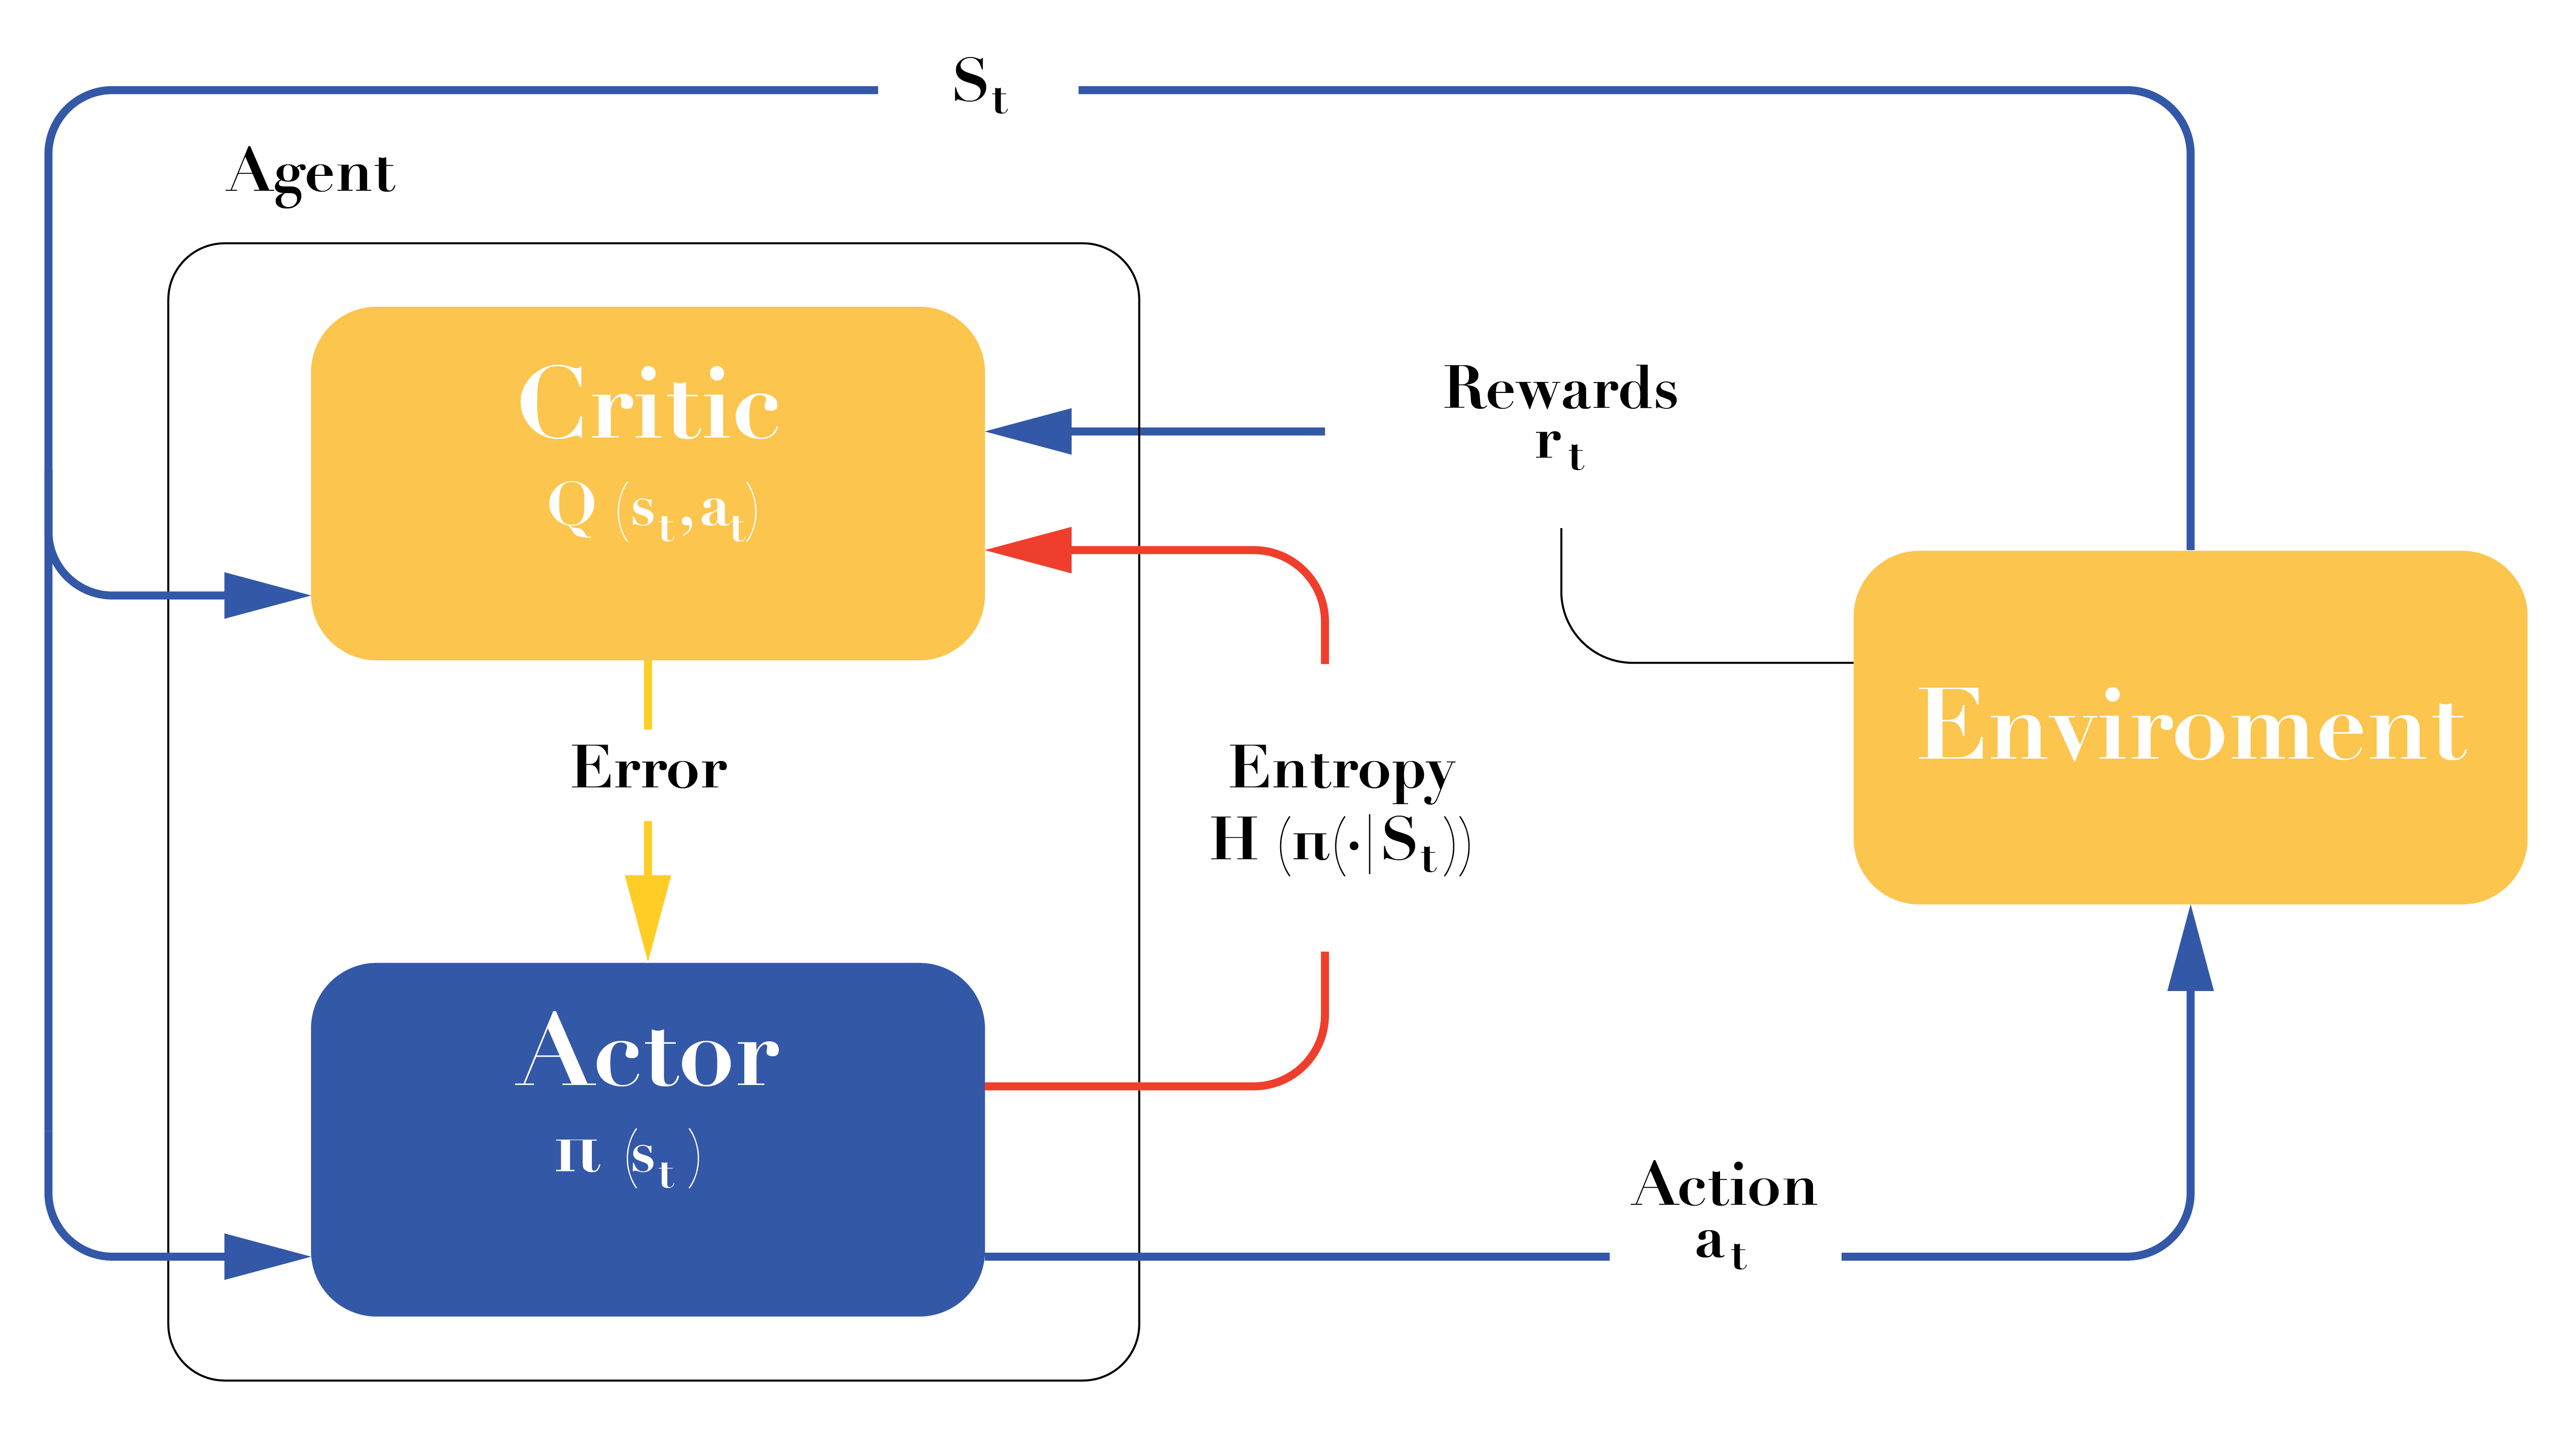
\includegraphics[width=0.6\textwidth]{background/sac.png}
  \end{center}
  \caption{Soft actor critic}
  \label{fig:sac}
\end{figure}

The maximum entropy framework used by SAC has several desirable properties. Firstly, it incentives a wider exploration during training. Secondly, the policy can capture multiple modes of near-optimal behavior. Lastly, it noticeably increases the learning speed over state-of-the-art methods that optimize the standard objective.

\section{Generative Adversarial Networks - GAN}
\begin{wrapfigure}{r}{0.6\textwidth}
  \begin{center}
    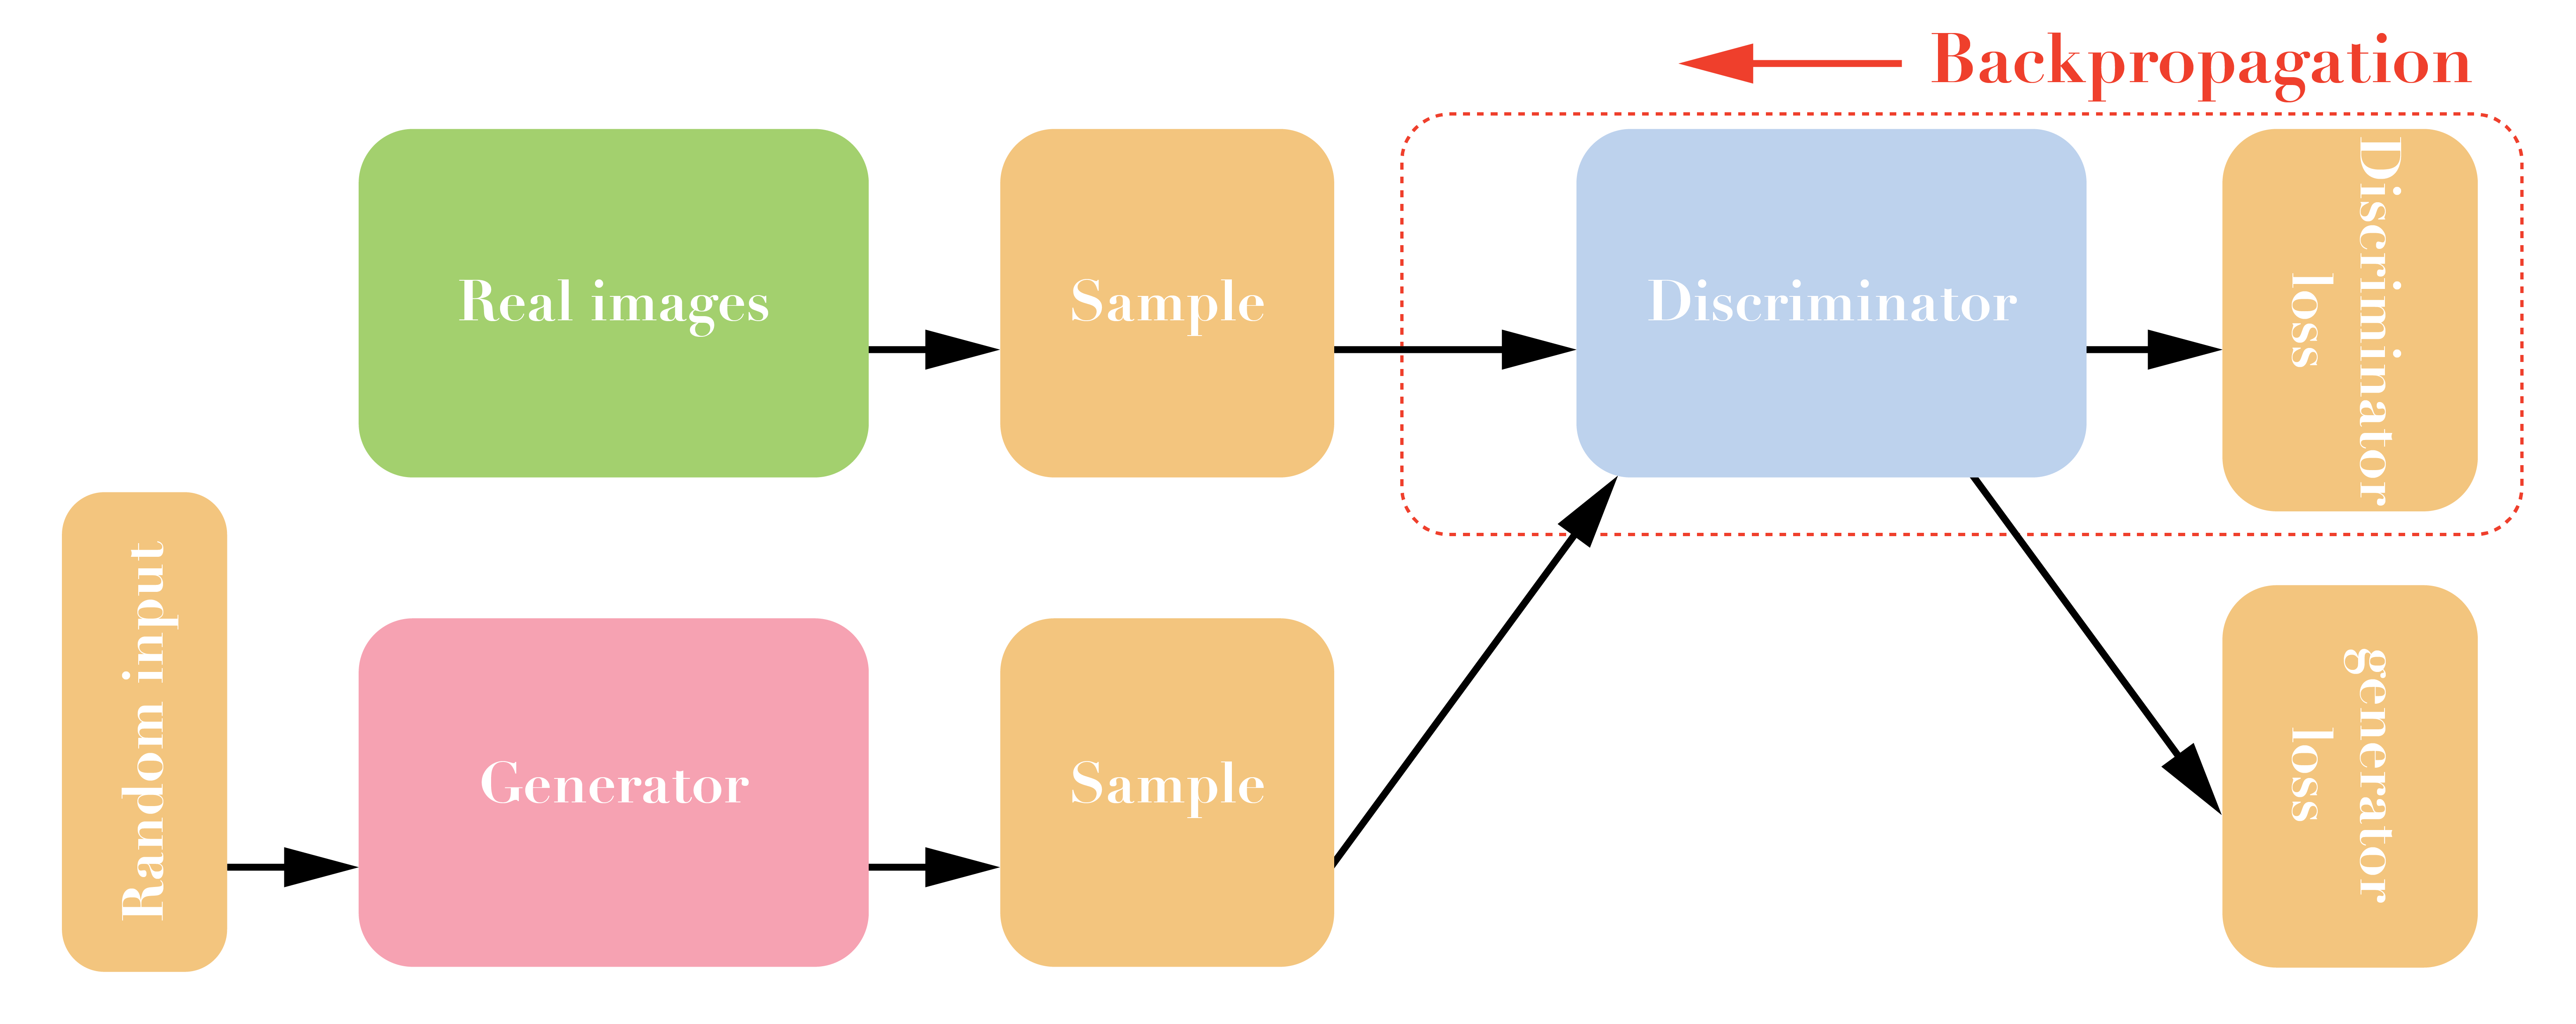
\includegraphics[width=0.6\textwidth]{background/gan.png}
  \end{center}
  \caption{GAN diagram}
  \label{fig:gan}
\end{wrapfigure}

Generative Adversarial Network is a framework introduced by \citet{art:gan} for training generative models in an unsupervised fashion. GANs can be used, for example, to generate visual paragraph \citep{Liang_2017_ICCV}, realistic text \citep{pmlr-v70-zhang17b}, photographs of human faces \citep{https://doi.org/10.48550/arxiv.1710.10196}, Image-to-Image translation \citep{Isola_2017_CVPR}.

The learning process involves two neural networks that are trained in an adversarial way, i.e. with an opposing objective.

Indeed, as described in Figure \ref{fig:gan}, the generator G generates inputs (e.g images) starting from random noise and the discriminator D needs to distinguish whether such inputs belong to the original dataset or not. GANs fall under the branch of unsupervised learning since the training process does not need labelled data as the generator is guided by the discriminator in order to generate inputs that resemble those of the original dataset.

$D$ is trained to maximize the probability of returning the correct label to both training examples and $G$ samples. At the same time $G$ attempt to minimize:
\begin{equation}
  \label{eq:gloss}
  L_G =log(1-D(G(z)))
\end{equation}

where $D(G(z))$ is the probability of $G(z)$ coming from the original dataset ($p_{X}$), then $1-D(G(z))$ defines the probability of $G(z)$ not coming from $p_{X}$. Since the generator wants to fool the discrimitar, it needs to minimize \ref{eq:gloss}.

In order to learn the generator's distribution $p_{g}$ over the training dataset $X$ such that $p_{g}\approx p_{X}$, a prior is defined on input noised variables $p_{z}(z)$, then it is mapped into the data space with the generator $G(z, \theta_{g})$. Beside that, the discriminator $D(x;\theta_{d})$, with $x \sim p_{g}$, outputs a single value which estimates the probability that $x$ came from the dataset $X$ rather than $p_{g}$. $D$ and $G$ are both differentiable function represented by a neural network with $\theta_{d}$ and $\theta_{g}$ respectively being their parameters.

In other words, the discriminator and the generator play a minimax game with the value function $V(G,D)$:
\begin{equation}
  \label{eq:ganloss}
  min_G max_D V(G,D) = \mathbb{E}_{x\sim \rho_{data}(x)}[log D(x)] + \mathbb{E}_{z\sim \rho_{z}(z)}[log (1-D(G(z)))]
\end{equation}

However, $G$ is initally weak since it has not learned a good $p_{g}$ yet, thus it cannot deceive the discriminator and $D$ can say with high confidence (probability close to 1) that $G(z)$ does not come from $p_{X}$ and therefore \ref{eq:gloss} would be at the minimum. To solve the aforementioned problem, \ref{eq:gloss} can be substituded with the maximization of the formula below in order to always have enough gradient:
\begin{equation}
  log(D(G(z)))
\end{equation}


\section{CycleGAN}
Image-To-Image translation is a complex task where the goal is to transform an image from one domain to another and viceversa, as shown in Figure \ref{fig:translation}.

\begin{wrapfigure}{r}{0.5\textwidth}
  \begin{center}
    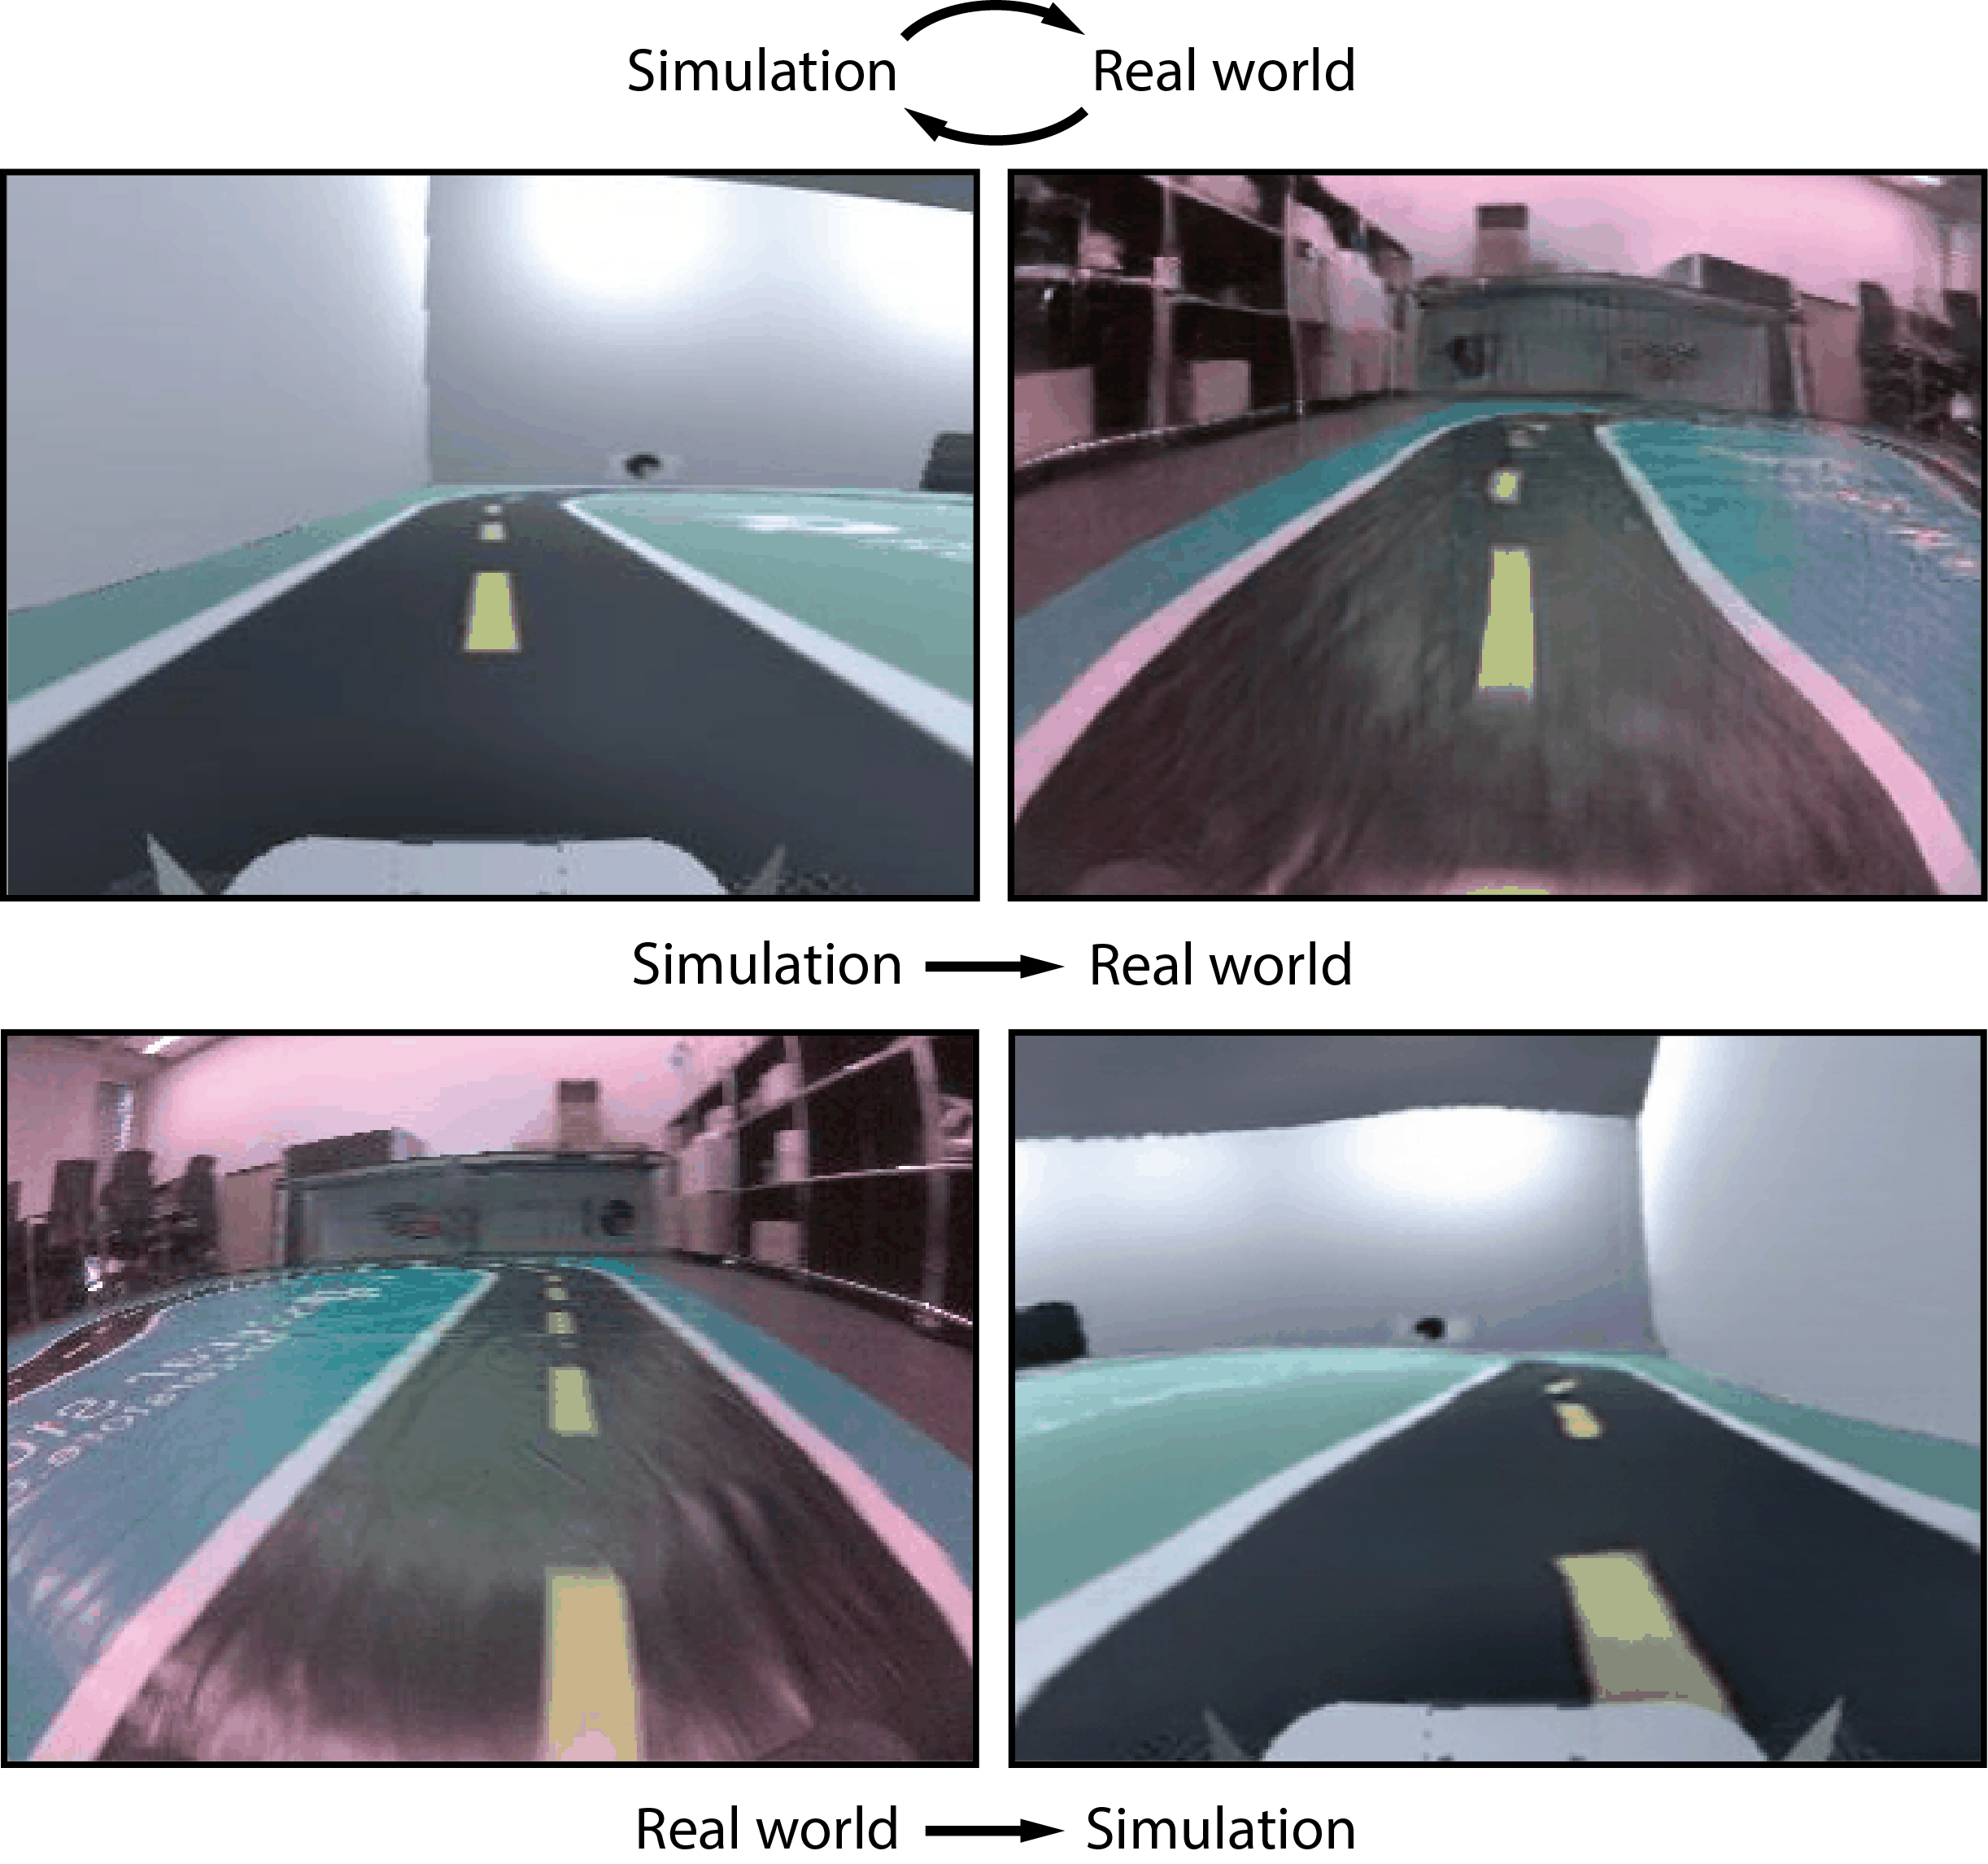
\includegraphics[width=0.5\textwidth]{background/imagetranslation.png}
  \end{center}
  \caption{Image-to-image translation example \citep{CycleGAN2017}.}
  \label{fig:translation}
\end{wrapfigure}
Prior papers have been presented to translate images, however they often require paired training examples between the domains [\citet{https://doi.org/10.48550/arxiv.1612.00835}, \citet{karakan}].
Such paired datasets can be very expensive or even impossible to gather, as in the case of object transfiguration ($horse \leftrightharpoons zebra$).

Cycle-Consistent Adversarial Networks from \citet{CycleGAN2017} (CycleGAN), aim to solve this problem in an unsupervised fashion. The main goal is to learn, using an adversarial loss, a mapping $G:X\rightarrow Y$ such that the image $G(x) $ with $x\in X$ is indistinguishable from a real image $y\in Y$. Since the mapping is highly under-costrained, an inverse mapping $F:Y \rightarrow X$ is introduced, together with a cycle-consistency loss to enforce $F(G(x)) \approx x$ and viceversa.
To accomplish the goal two discriminator $D_{X}$ and $D_{Y}$ are provided. $D_{X}$ tries to distinguish between training samples $\rho_{data}(X)$ and their translations $F(Y)$ and viceversa for $D_{Y}$. 
The full objective \ref{eq:cycleganloss} includes the adversarial losses and the cycle-consistency loss to encourage a consistent translation from one domain to the other:
\begin{equation}
  \label{eq:cycleganloss}
  L(G,F,D_{X}, D_{Y}) = L_{GAN}(G, D_{Y},X,Y) + L_{GAN}(F, D_{X},Y,X) + \lambda L_{cyc}(G,F)
\end{equation}
where the loss $L_{GAN}(G, D_{Y},X,Y)$ and $L_{GAN}(F, D_{X},Y,X)$ are described in \ref{eq:ganloss} from standard GANs
% where the loss $L_{GAN}(G, D_{Y},X,Y)$ is described below and $L_{GAN}(F, D_{X},Y,X)$ can be derived similarly:
% \begin{equation}
% L_{GAN}(G, D_{Y},X,Y) = \mathbb{E}_{y\sim \rho_{data}(y)}[log D_{Y}(y)] + \mathbb{E}_{x\sim \rho_{data}(x)}[log (1-D_{Y}(G(x)))]
% \end{equation}
and the following is the cycle-consistency loss:
\begin{equation}
  L_{cyc}(G,F) =  \mathbb{E}_{x\sim \rho_{data}(x)}[\left \| F(G(X))-x \right \|_1] + \mathbb{E}_{y\sim \rho_{data}(y)}[\left \| G(F(y))-y \right \|_1]
\end{equation}
where $\lambda$ is a temperature parameter to define the importance of such loss in Equation \ref{eq:cycleganloss} and $\| \cdot \|_1$ is the L1 norm or rather the sum of the magnitudes of the vectors in a space, a measure of the distance between vectors.

\section{AutoEncoder and Variational AutoEncoder}

\subsection{AutoEncoder}
AutoEncoders (AEs) are artificial neural networks that fall under the branch of unsupervised learning since they learn efficient encoding into a latent space without the supervision of labelled data. They are generally used for vary purposes, for example, dimensionality reduction, image compression, image denoising, image generation, feature extraction and sentence generation [\citet{doi:10.1126/science.1127647}, \citet{8456308}, \citet{7836672}, \citet{7926714}, \citet{8852155}]. 

Taking as example the case of image dimensionality reduction, an AE is composed of two main parts, an encoder $E$ and a decoder $D$. 
\begin{align}
  E_\phi &:  X \rightarrow Z & D_\theta &:  Z \rightarrow X^{'}
\end{align}
where $X = \mathbb{R}^{mxn}$ and $Z = \mathbb{R}^{k }$ for some $m,n,k$ and $k\ll mxn$ to reach the goal of dimensionality reduction. The optimal case is reached when $X=X^{'} $. They are both parametrized function with $\phi$ and $\theta$ being respectively their parameters, to put it another way the parameters of the neural networks, generally multilayer perceptrons, of which they are composed of.
As shown in Figure \ref{fig:ae}, the main goal of the encoder is to learn a mapping of each observation of the dataset $x \in X$ into a latent space of smaller dimensionality.  Since a label is not available, in order to measure the quality of the embedded image into the latent space, the decoder is used to reconstruct to image and then compute the loss.

\begin{figure}[h]
  \begin{center}
    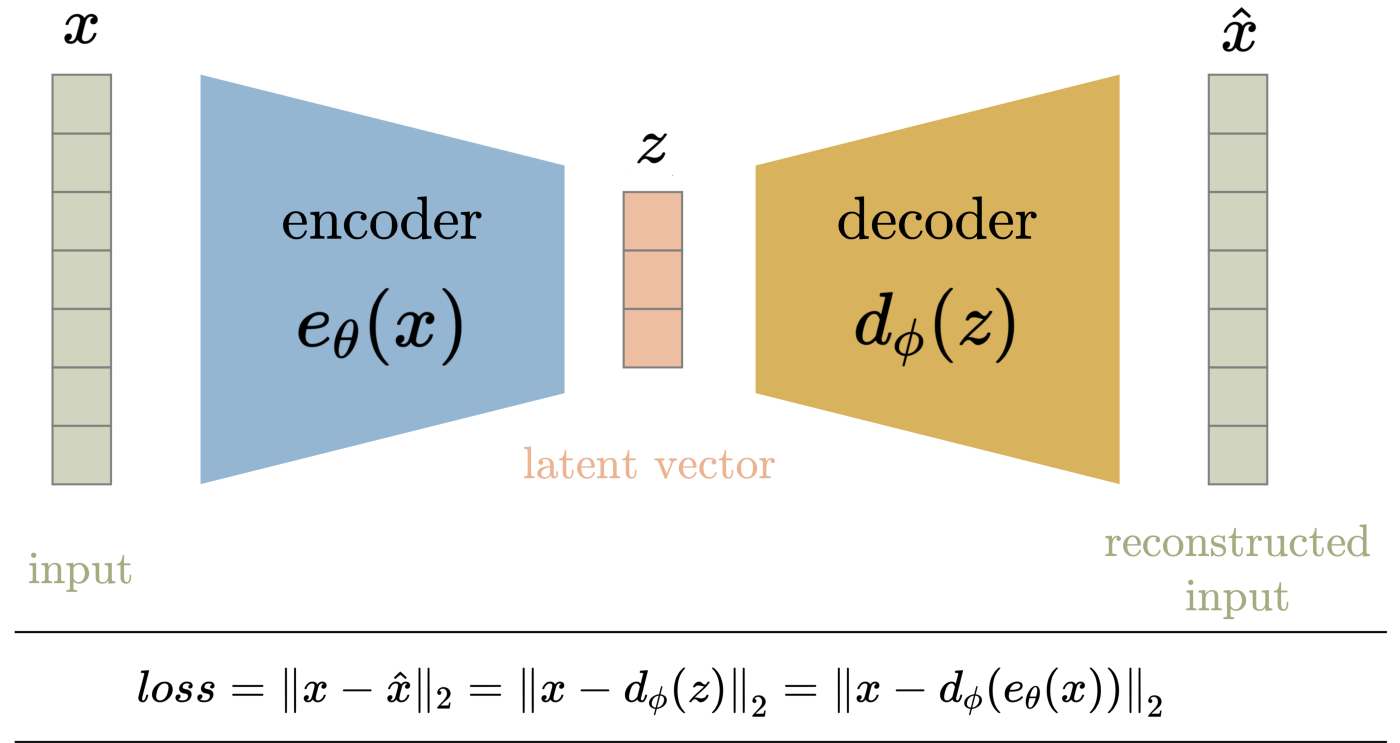
\includegraphics[width=0.70\textwidth]{background/ae.png}
  \end{center}
  \caption{AE diagram}
  \label{fig:ae}
\end{figure}

In other words, the encoder maps an image $x\in X$ into the latent space producing ${z=E_{\phi }(x)}$ with $z\in Z$, then $z$ is reconstructed by the decoder to bring it back to the orginal space ${x'=D_{\theta }(z)}$ with $x^{'}\in X^{'}$. Finally, $x^{'}$ can be used as a label with any distance measure $d(x,x^{'})$. Thus the loss to be minimized is so computed:

\begin{equation}
\label{eq:aeloss}
  L(\theta ,\phi ) = d(x_{i},D_{\theta }(E_{\phi }(x_{i})))
\end{equation}

\begin{figure}[h]
  \begin{minipage}{.5\textwidth}
    \centering
    \captionsetup{margin=0.8cm}
    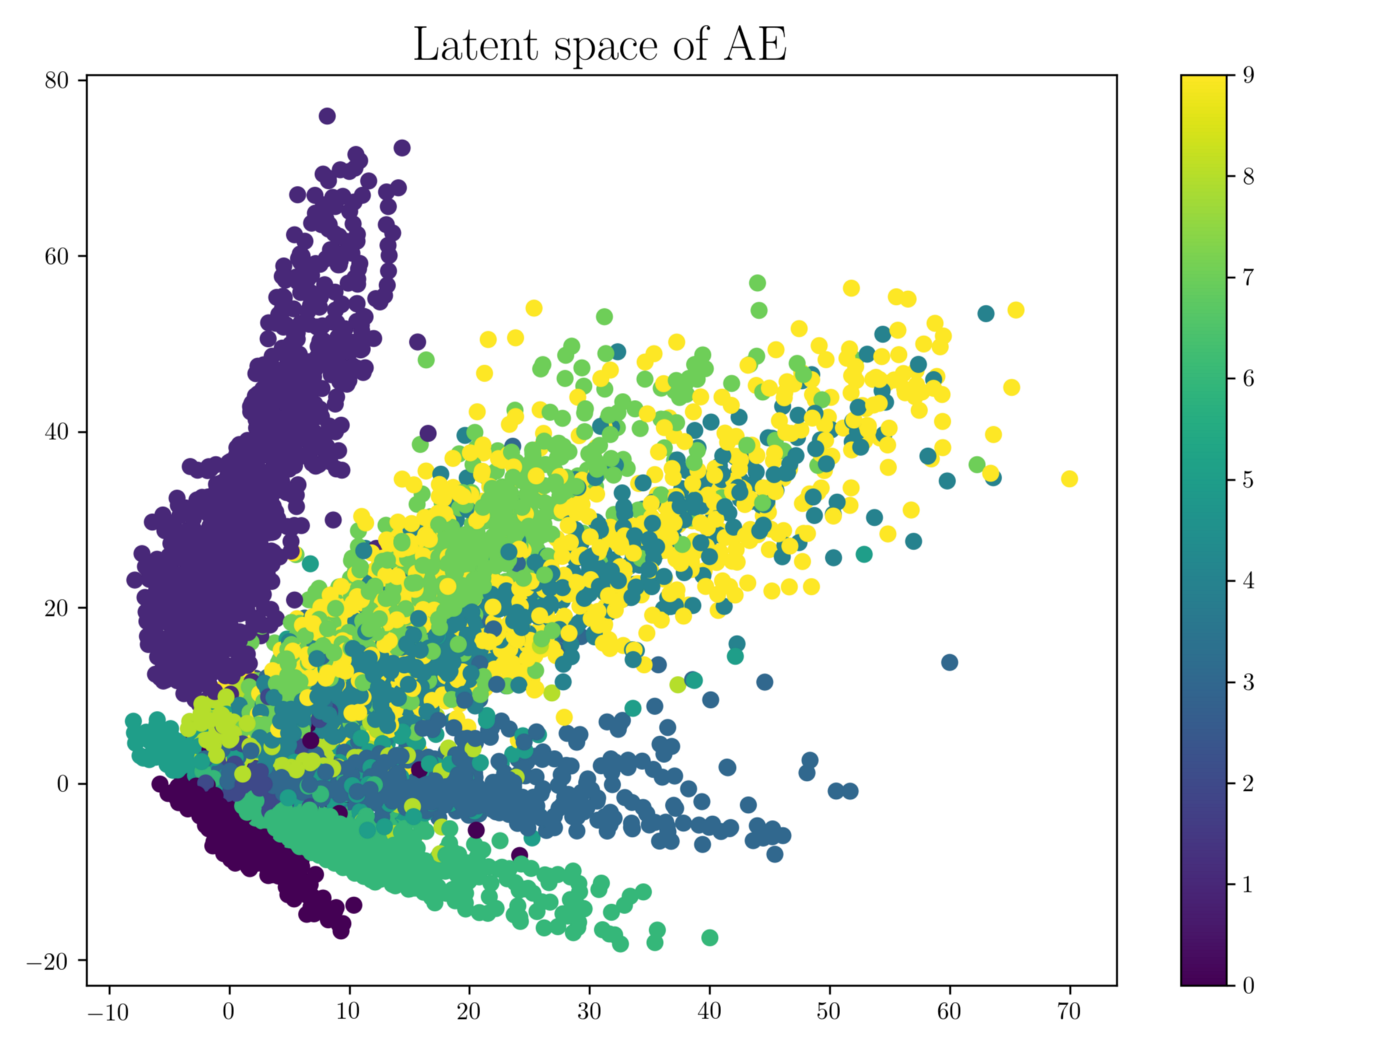
\includegraphics[width=0.95\textwidth]{background/latentspace.png}
    \captionof{figure}{Example AE latent space $Z$ on MNIST datasetk}
    \label{fig:latent}
  \end{minipage}%
  \begin{minipage}{.5\textwidth}
      \centering
      \captionsetup{margin=0.8cm}
      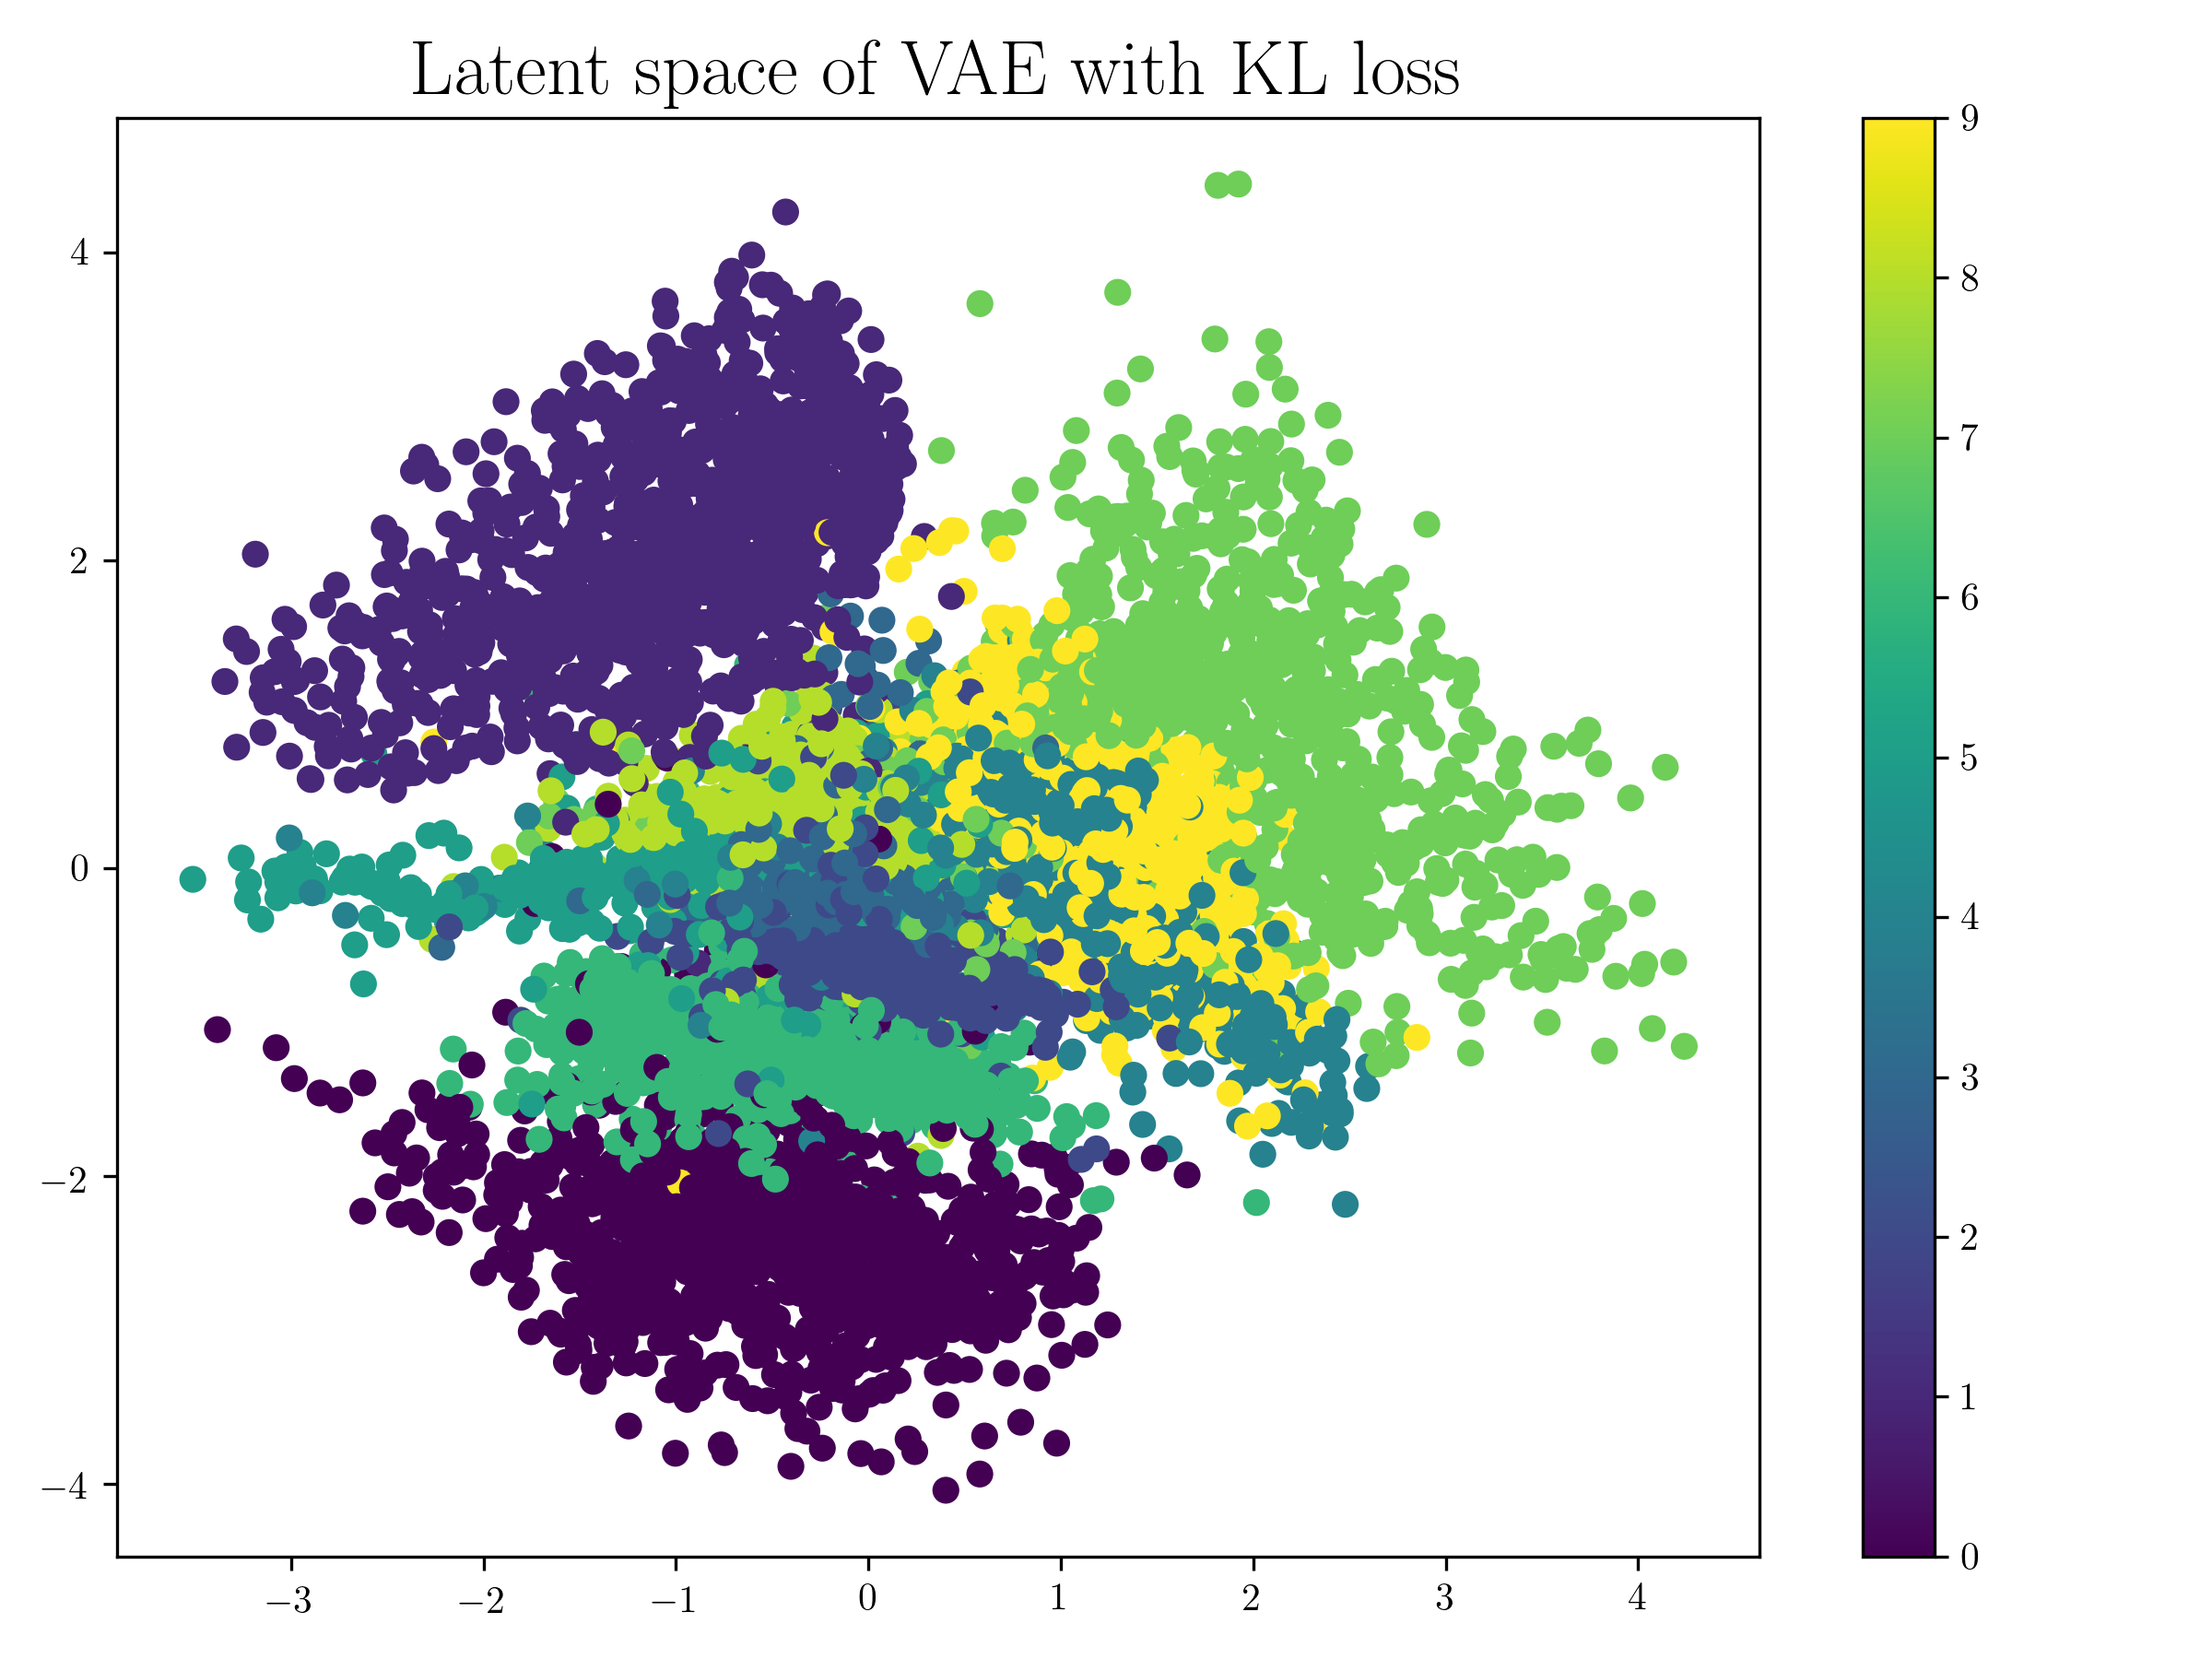
\includegraphics[width=0.95\textwidth]{background/vaelatentspace.png}
      \captionof{figure}{Example VAE latent space $Z$ on MNIST dataset}
      \label{fig:vaelatent}
  \end{minipage}
\end{figure}

In Figure \ref{fig:latent} is shown a typical example of how the MNIST dataset looks like once mapped into the latent space. After the AE is trained, a random generated observation could be given to it to generate a new sample from the dataset distribution. However, there are parts of the latent space that does not correspond to any data point. Thus using sample from the \textit{white space} will not generate any meaningful image. That is why a basic so-designed AE cannot be used as a general generative model, eventhough a random sample that falls into any cluster in the latent space can certainly produce a meaningful image, also an image never seen in training even if only with small variations. 

AEs, results to be much more capable in data compression since the latent space of a linear autoencoder strongly resembles the eigenspace achieved during the principal component analysis of the data, with the added value of the non-linearity. Thus making AEs capable of learning rather powerful representations of the input data in lower dimensions with much less information loss.


\subsection{Variational AutoEncoder}

Variational AutoEncoders (VAEs) addresses the problem of \textit{strong localization} of data point into the latent space thus providing a more powerful generative capability then AEs.

\begin{figure}[h]
  \begin{center}
    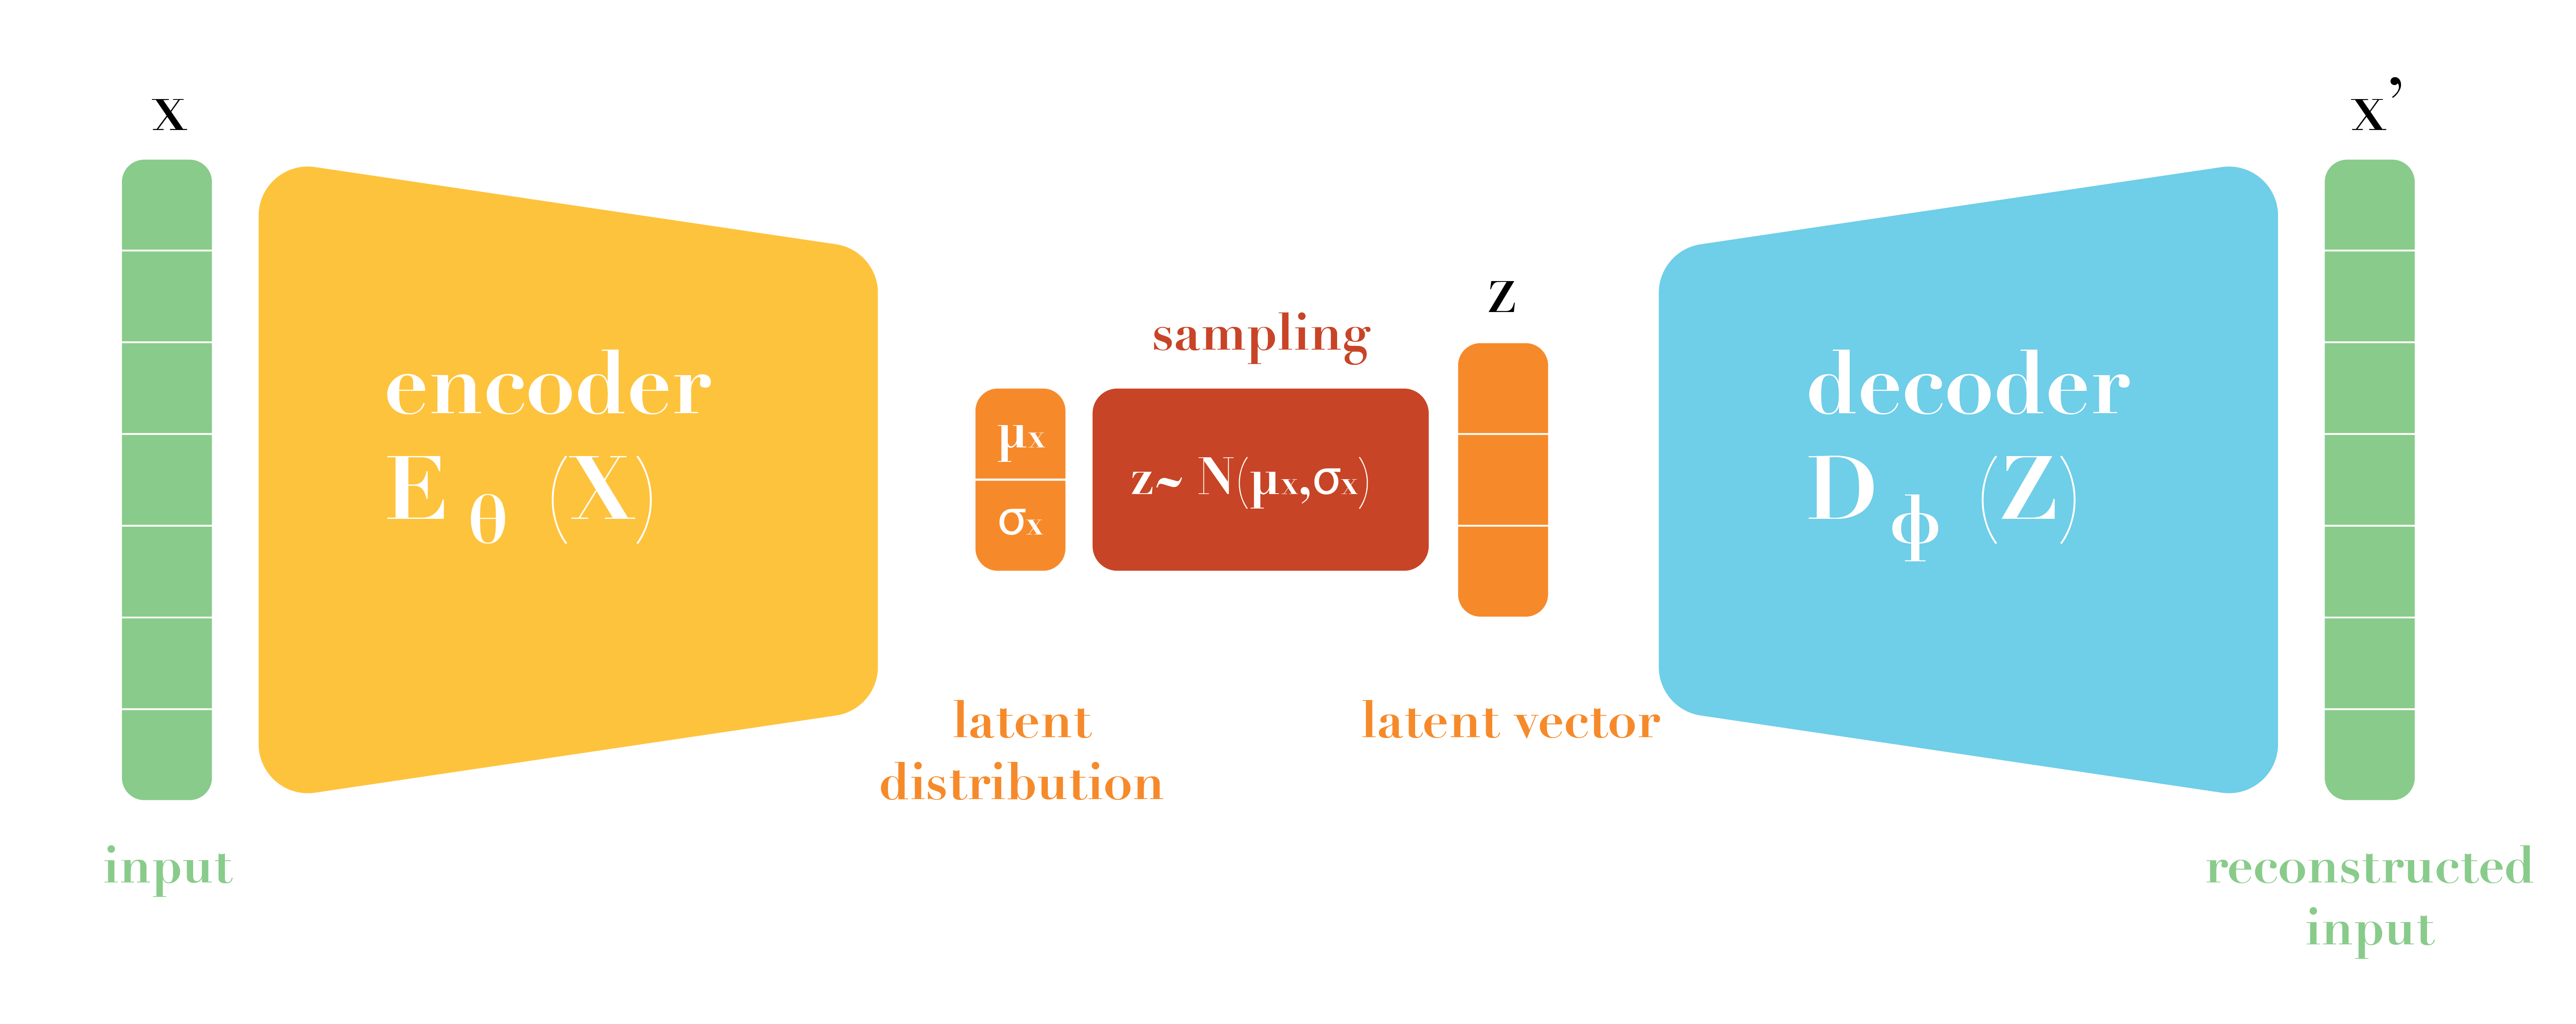
\includegraphics[width=0.80\textwidth]{background/vae.png}
  \end{center}
  \caption{VAE diagram}
  \label{fig:vae}
\end{figure}

As shown in Figure \ref{fig:vae} only a small change with respect to AEs is introduced, the encoder instead of mapping directly samples into the latent space outputs parameters of a pre-defined distribution (usually Normal) in the latent space for every input. Then $z$ is produced by sampling from a normal distribution with the outputted parameters. 

In other words, the encoder, starting from an image $x\in X$, produces the gaussian parameters ${[\mu_x, \sigma_x]=E_{\phi }(x)}$, then $z$ is sampled from a normal distribution $z \sim \mathcal{N}(\mu_x, \sigma_x)$. Consequently, the decoder brings it back to the orginal space ${x'=D_{\theta }(z)}$ with $x^{'}\in X^{'}$. Finally, $x^{'}$ can be used as a label with any distance measure $d(x,x^{'})$. Thus the loss to be minimized is so computed:
\begin{equation}
\label{eq:vaeloss}
  L(\theta ,\phi) = d(x_{i},D_{\theta }(E_{\phi }(x_{i}))) + KL[\mathcal{N} (\mu_x, \sigma_x),\mathcal{N}(0, 1)]
\end{equation}
where the firs term is equivalent to \ref{eq:aeloss} and KL is the Kulback-Leibler divergence, a measure of how one probability distribution is different from another. The KL divergence acts as a regularization term by enforcing predicted distributions to be close to the identity, giving to the latent space two main properties, continuity (close points in the latent space should be close also when decoded) and completeness (any point sampled from the latent space should always be meaningful once decoded) as shown in Figure \ref{fig:vaelatent}.

\section{DonkeyCar} \label{sec:donkeycar}
DonkeyCar, shown in Figure \ref{fig:donkey}, is an open source DIY platform providing software and hardware tools for the development of self-driving car algorithms. The basic car is a simple remote controlled car that can be 3D printed or bought as a kit for a reasonable and affordable price. The main models recommended by the official documentation are:

\begin{itemize}
  \item Exceed Magnet Blue, Red
  \item Exceed Desert Monster Green
  \item Exceed Short Course Truck Green, Red
  \item Exceed Blaze Blue, Yellow, Wild Blue, Max Red
\end{itemize}

These cars are electrically identical but have different tires and mounting. They are also equipped with brushed motors which make ML training easier since they handle rough driving surfaces well and are inexpensive. The car can be customized with additional sensors as LIDARs and IMUs to provide more information about the surroundings of the car.

\begin{wrapfigure}[19]{r}{0.5\textwidth}
  \begin{center}
    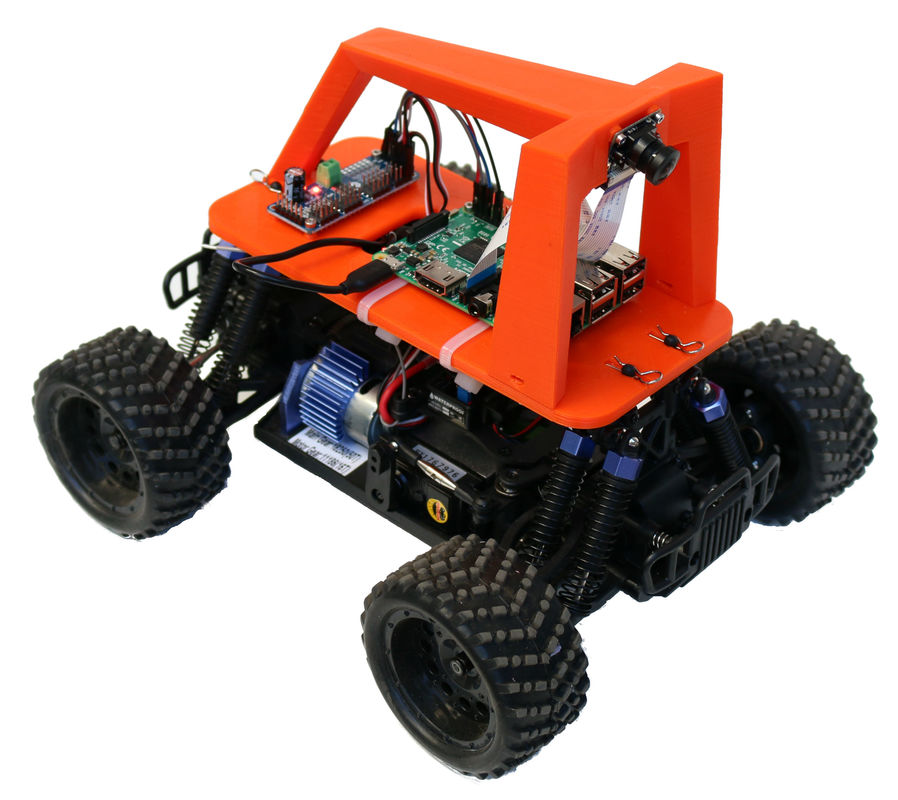
\includegraphics[width=0.5\textwidth]{background/donkey.jpeg}
  \end{center}
  \caption{Assembled donkeycar}
  \label{fig:donkey}
\end{wrapfigure}

In particular, the car used for the purposes of this thesis, is a basic donkey car equipped with an 8-megapixel IMX219 sensor that features an 160 degree field of view. It is capable of taking photos with a resolution of 3280x2464 and video recording up to a resolution of 1080p at 30 frames per seconds. In order to process all the information coming from the camera, control the motors and run the self-driving car softwarethe self-driving car software it is equipped with an NVIDIA Jetson Nano microcontroller. To power comes from a LiPO battery 11.1V and 2200mAh that powers the electric motor and the microcontroller. Additionally, to expand the operational life of the car, a power-bank can be added to exclusively power the microcontroller, while the LiPO battery is dedicated at powering the engine. 
A DonkeyCar can be remotely controlled either with a joypad or directly by the software.